\documentclass{article}
\usepackage{amsfonts}
\usepackage{amsmath}
\usepackage{amssymb}
\usepackage[utf8]{inputenc}
\usepackage{graphicx}
\graphicspath{{./images/}}

\title{
    ECE-345: VLSI \\ 
    Chapter 1: Frequency Response Model
}
\author{Amaan Rahman}

\begin{document}
\maketitle
\section{Preliminary Concepts}
\subsection{Bipolar Amplifiers}
\subsubsection{Large Signal Model}
Collector current: $I_C = I_S\,\text{exp}\left(\frac{V_{BE}}{V_T}\right)$ \\
Collector, Base, Emitter current relations: 
\begin{equation*}
    \begin{split}
        I_C &= \beta I_B = \frac{\beta}{\beta + 1}I_E\\
        I_E &= I_C + I_B = I_C\left(1 + \frac{1}{\beta}\right) \\
        &\therefore \\
        I_C &= I_S\,\text{exp}\left(\frac{V_{BE}}{V_T}\right) \\
        I_B &= \frac{1}{\beta}I_S\,\text{exp}\left(\frac{V_{BE}}{V_T}\right) \\
        I_E &= \frac{\beta + 1}{\beta}I_S\,\text{exp}\left(\frac{V_{BE}}{V_T}\right)
    \end{split}
\end{equation*}

\subsubsection{Small Signal Model}
Transconductance: $g_m = \frac{I_C}{V_T}$ \\
Base-Emitter resistance: $r_{\pi} = \frac{\beta}{g_m}$ \\
Introducing \textbf{Early Effect}: 
\begin{equation*}
    \begin{split}
        I_C &= \left(I_S\,\text{exp}\left(\frac{V_{BE}}{V_T}\right)\right)\left(1 + \frac{V_{CE}}{V_A}\right) \\
        r_O &= \frac{V_A}{I_C}
    \end{split}
\end{equation*}
\subsubsection{Amplifier Topologies}
\textit{Common-Emitter Topology (w/ Emitter Degeneration):} \\
\begin{tabular}{ccc}
    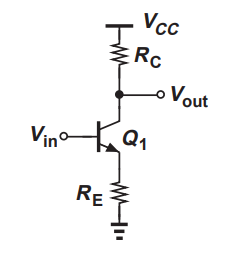
\includegraphics[scale=0.5]{CE_top.png} & \
    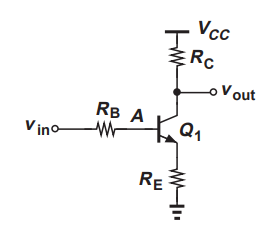
\includegraphics[scale=0.53]{CE_Rb_top.png} \\

    \parbox{6cm}{
        \begin{equation*}
            \begin{split}
                R_{in} &= r_{\pi} + (\beta + 1)R_E \\
                R_{out} &= \left(1 + g_m R_E\right)r_O \\
                A_v &= -\frac{R_C}{\frac{1}{g_m} + R_E}
            \end{split}
        \end{equation*}
    } & \parbox{6cm}{
        \begin{equation*}
            \begin{split}
                R_{in} &= R_B + r_{\pi} + (\beta + 1)R_E \\
                R_{out} &= \left(1 + g_m R_E\right)r_O \\
                A_v &= -\frac{R_C \parallel r_O}{\frac{1}{g_m} + R_E}
            \end{split}
        \end{equation*}
    } 
\end{tabular}
\subsection{CMOS Amplifiers}


\end{document}
